
%% bare_jrnl.tex
%% V1.3
%% 2007/01/11
%% by Michael Shell
%% see http://www.michaelshell.org/
%% for current contact information.
%%
%% This is a skeleton file demonstrating the use of IEEEtran.cls
%% (requires IEEEtran.cls version 1.7 or later) with an IEEE journal paper.
%%
%% Support sites:
%% http://www.michaelshell.org/tex/ieeetran/
%% http://www.ctan.org/tex-archive/macros/latex/contrib/IEEEtran/
%% and
%% http://www.ieee.org/



% *** Authors should verify (and, if needed, correct) their LaTeX system  ***
% *** with the testflow diagnostic prior to trusting their LaTeX platform ***
% *** with production work. IEEE's font choices can trigger bugs that do  ***
% *** not appear when using other class files.                            ***
% The testflow support page is at:
% http://www.michaelshell.org/tex/testflow/


%%*************************************************************************
%% Legal Notice:
%% This code is offered as-is without any warranty either expressed or
%% implied; without even the implied warranty of MERCHANTABILITY or
%% FITNESS FOR A PARTICULAR PURPOSE! 
%% User assumes all risk.
%% In no event shall IEEE or any contributor to this code be liable for
%% any damages or losses, including, but not limited to, incidental,
%% consequential, or any other damages, resulting from the use or misuse
%% of any information contained here.
%%
%% All comments are the opinions of their respective authors and are not
%% necessarily endorsed by the IEEE.
%%
%% This work is distributed under the LaTeX Project Public License (LPPL)
%% ( http://www.latex-project.org/ ) version 1.3, and may be freely used,
%% distributed and modified. A copy of the LPPL, version 1.3, is included
%% in the base LaTeX documentation of all distributions of LaTeX released
%% 2003/12/01 or later.
%% Retain all contribution notices and credits.
%% ** Modified files should be clearly indicated as such, including  **
%% ** renaming them and changing author support contact information. **
%%
%% File list of work: IEEEtran.cls, IEEEtran_HOWTO.pdf, bare_adv.tex,
%%                    bare_conf.tex, bare_jrnl.tex, bare_jrnl_compsoc.tex
%%*************************************************************************

% Note that the a4paper option is mainly intended so that authors in
% countries using A4 can easily print to A4 and see how their papers will
% look in print - the typesetting of the document will not typically be
% affected with changes in paper size (but the bottom and side margins will).
% Use the testflow package mentioned above to verify correct handling of
% both paper sizes by the user's LaTeX system.
%
% Also note that the "draftcls" or "draftclsnofoot", not "draft", option
% should be used if it is desired that the figures are to be displayed in
% draft mode.
%
\documentclass[journal]{IEEEtran}
\usepackage{blindtext}
\usepackage{graphicx}
\usepackage{hyperref}
\usepackage{float}


% Some very useful LaTeX packages include:
% (uncomment the ones you want to load)


% *** MISC UTILITY PACKAGES ***
%
%\usepackage{ifpdf}
% Heiko Oberdiek's ifpdf.sty is very useful if you need conditional
% compilation based on whether the output is pdf or dvi.
% usage:
% \ifpdf
%   % pdf code
% \else
%   % dvi code
% \fi
% The latest version of ifpdf.sty can be obtained from:
% http://www.ctan.org/tex-archive/macros/latex/contrib/oberdiek/
% Also, note that IEEEtran.cls V1.7 and later provides a builtin
% \ifCLASSINFOpdf conditional that works the same way.
% When switching from latex to pdflatex and vice-versa, the compiler may
% have to be run twice to clear warning/error messages.






% *** CITATION PACKAGES ***
%
%\usepackage{cite}
% cite.sty was written by Donald Arseneau
% V1.6 and later of IEEEtran pre-defines the format of the cite.sty package
% \cite{} output to follow that of IEEE. Loading the cite package will
% result in citation numbers being automatically sorted and properly
% "compressed/ranged". e.g., [1], [9], [2], [7], [5], [6] without using
% cite.sty will become [1], [2], [5]--[7], [9] using cite.sty. cite.sty's
% \cite will automatically add leading space, if needed. Use cite.sty's
% noadjust option (cite.sty V3.8 and later) if you want to turn this off.
% cite.sty is already installed on most LaTeX systems. Be sure and use
% version 4.0 (2003-05-27) and later if using hyperref.sty. cite.sty does
% not currently provide for hyperlinked citations.
% The latest version can be obtained at:
% http://www.ctan.org/tex-archive/macros/latex/contrib/cite/
% The documentation is contained in the cite.sty file itself.






% *** GRAPHICS RELATED PACKAGES ***
%
\ifCLASSINFOpdf
  % \usepackage[pdftex]{graphicx}
  % declare the path(s) where your graphic files are
  % \graphicspath{{../pdf/}{../jpeg/}}
  % and their extensions so you won't have to specify these with
  % every instance of \includegraphics
  % \DeclareGraphicsExtensions{.pdf,.jpeg,.png}
\else
  % or other class option (dvipsone, dvipdf, if not using dvips). graphicx
  % will default to the driver specified in the system graphics.cfg if no
  % driver is specified.
  % \usepackage[dvips]{graphicx}
  % declare the path(s) where your graphic files are
  % \graphicspath{{../eps/}}
  % and their extensions so you won't have to specify these with
  % every instance of \includegraphics
  % \DeclareGraphicsExtensions{.eps}
\fi
% graphicx was written by David Carlisle and Sebastian Rahtz. It is
% required if you want graphics, photos, etc. graphicx.sty is already
% installed on most LaTeX systems. The latest version and documentation can
% be obtained at: 
% http://www.ctan.org/tex-archive/macros/latex/required/graphics/
% Another good source of documentation is "Using Imported Graphics in
% LaTeX2e" by Keith Reckdahl which can be found as epslatex.ps or
% epslatex.pdf at: http://www.ctan.org/tex-archive/info/
%
% latex, and pdflatex in dvi mode, support graphics in encapsulated
% postscript (.eps) format. pdflatex in pdf mode supports graphics
% in .pdf, .jpeg, .png and .mps (metapost) formats. Users should ensure
% that all non-photo figures use a vector format (.eps, .pdf, .mps) and
% not a bitmapped formats (.jpeg, .png). IEEE frowns on bitmapped formats
% which can result in "jaggedy"/blurry rendering of lines and letters as
% well as large increases in file sizes.
%
% You can find documentation about the pdfTeX application at:
% http://www.tug.org/applications/pdftex





% *** MATH PACKAGES ***
%
%\usepackage[cmex10]{amsmath}
% A popular package from the American Mathematical Society that provides
% many useful and powerful commands for dealing with mathematics. If using
% it, be sure to load this package with the cmex10 option to ensure that
% only type 1 fonts will utilized at all point sizes. Without this option,
% it is possible that some math symbols, particularly those within
% footnotes, will be rendered in bitmap form which will result in a
% document that can not be IEEE Xplore compliant!
%
% Also, note that the amsmath package sets \interdisplaylinepenalty to 10000
% thus preventing page breaks from occurring within multiline equations. Use:
%\interdisplaylinepenalty=2500
% after loading amsmath to restore such page breaks as IEEEtran.cls normally
% does. amsmath.sty is already installed on most LaTeX systems. The latest
% version and documentation can be obtained at:
% http://www.ctan.org/tex-archive/macros/latex/required/amslatex/math/





% *** SPECIALIZED LIST PACKAGES ***
%
%\usepackage{algorithmic}
% algorithmic.sty was written by Peter Williams and Rogerio Brito.
% This package provides an algorithmic environment fo describing algorithms.
% You can use the algorithmic environment in-text or within a figure
% environment to provide for a floating algorithm. Do NOT use the algorithm
% floating environment provided by algorithm.sty (by the same authors) or
% algorithm2e.sty (by Christophe Fiorio) as IEEE does not use dedicated
% algorithm float types and packages that provide these will not provide
% correct IEEE style captions. The latest version and documentation of
% algorithmic.sty can be obtained at:
% http://www.ctan.org/tex-archive/macros/latex/contrib/algorithms/
% There is also a support site at:
% http://algorithms.berlios.de/index.html
% Also of interest may be the (relatively newer and more customizable)
% algorithmicx.sty package by Szasz Janos:
% http://www.ctan.org/tex-archive/macros/latex/contrib/algorithmicx/




% *** ALIGNMENT PACKAGES ***
%
%\usepackage{array}
% Frank Mittelbach's and David Carlisle's array.sty patches and improves
% the standard LaTeX2e array and tabular environments to provide better
% appearance and additional user controls. As the default LaTeX2e table
% generation code is lacking to the point of almost being broken with
% respect to the quality of the end results, all users are strongly
% advised to use an enhanced (at the very least that provided by array.sty)
% set of table tools. array.sty is already installed on most systems. The
% latest version and documentation can be obtained at:
% http://www.ctan.org/tex-archive/macros/latex/required/tools/


%\usepackage{mdwmath}
%\usepackage{mdwtab}
% Also highly recommended is Mark Wooding's extremely powerful MDW tools,
% especially mdwmath.sty and mdwtab.sty which are used to format equations
% and tables, respectively. The MDWtools set is already installed on most
% LaTeX systems. The lastest version and documentation is available at:
% http://www.ctan.org/tex-archive/macros/latex/contrib/mdwtools/


% IEEEtran contains the IEEEeqnarray family of commands that can be used to
% generate multiline equations as well as matrices, tables, etc., of high
% quality.


%\usepackage{eqparbox}
% Also of notable interest is Scott Pakin's eqparbox package for creating
% (automatically sized) equal width boxes - aka "natural width parboxes".
% Available at:
% http://www.ctan.org/tex-archive/macros/latex/contrib/eqparbox/





% *** SUBFIGURE PACKAGES ***
%\usepackage[tight,footnotesize]{subfigure}
% subfigure.sty was written by Steven Douglas Cochran. This package makes it
% easy to put subfigures in your figures. e.g., "Figure 1a and 1b". For IEEE
% work, it is a good idea to load it with the tight package option to reduce
% the amount of white space around the subfigures. subfigure.sty is already
% installed on most LaTeX systems. The latest version and documentation can
% be obtained at:
% http://www.ctan.org/tex-archive/obsolete/macros/latex/contrib/subfigure/
% subfigure.sty has been superceeded by subfig.sty.



%\usepackage[caption=false]{caption}
%\usepackage[font=footnotesize]{subfig}
% subfig.sty, also written by Steven Douglas Cochran, is the modern
% replacement for subfigure.sty. However, subfig.sty requires and
% automatically loads Axel Sommerfeldt's caption.sty which will override
% IEEEtran.cls handling of captions and this will result in nonIEEE style
% figure/table captions. To prevent this problem, be sure and preload
% caption.sty with its "caption=false" package option. This is will preserve
% IEEEtran.cls handing of captions. Version 1.3 (2005/06/28) and later 
% (recommended due to many improvements over 1.2) of subfig.sty supports
% the caption=false option directly:
%\usepackage[caption=false,font=footnotesize]{subfig}
%
% The latest version and documentation can be obtained at:
% http://www.ctan.org/tex-archive/macros/latex/contrib/subfig/
% The latest version and documentation of caption.sty can be obtained at:
% http://www.ctan.org/tex-archive/macros/latex/contrib/caption/




% *** FLOAT PACKAGES ***
%
%\usepackage{fixltx2e}
% fixltx2e, the successor to the earlier fix2col.sty, was written by
% Frank Mittelbach and David Carlisle. This package corrects a few problems
% in the LaTeX2e kernel, the most notable of which is that in current
% LaTeX2e releases, the ordering of single and double column floats is not
% guaranteed to be preserved. Thus, an unpatched LaTeX2e can allow a
% single column figure to be placed prior to an earlier double column
% figure. The latest version and documentation can be found at:
% http://www.ctan.org/tex-archive/macros/latex/base/



%\usepackage{stfloats}
% stfloats.sty was written by Sigitas Tolusis. This package gives LaTeX2e
% the ability to do double column floats at the bottom of the page as well
% as the top. (e.g., "\begin{figure*}[!b]" is not normally possible in
% LaTeX2e). It also provides a command:
%\fnbelowfloat
% to enable the placement of footnotes below bottom floats (the standard
% LaTeX2e kernel puts them above bottom floats). This is an invasive package
% which rewrites many portions of the LaTeX2e float routines. It may not work
% with other packages that modify the LaTeX2e float routines. The latest
% version and documentation can be obtained at:
% http://www.ctan.org/tex-archive/macros/latex/contrib/sttools/
% Documentation is contained in the stfloats.sty comments as well as in the
% presfull.pdf file. Do not use the stfloats baselinefloat ability as IEEE
% does not allow \baselineskip to stretch. Authors submitting work to the
% IEEE should note that IEEE rarely uses double column equations and
% that authors should try to avoid such use. Do not be tempted to use the
% cuted.sty or midfloat.sty packages (also by Sigitas Tolusis) as IEEE does
% not format its papers in such ways.


%\ifCLASSOPTIONcaptionsoff
%  \usepackage[nomarkers]{endfloat}
% \let\MYoriglatexcaption\caption
% \renewcommand{\caption}[2][\relax]{\MYoriglatexcaption[#2]{#2}}
%\fi
% endfloat.sty was written by James Darrell McCauley and Jeff Goldberg.
% This package may be useful when used in conjunction with IEEEtran.cls'
% captionsoff option. Some IEEE journals/societies require that submissions
% have lists of figures/tables at the end of the paper and that
% figures/tables without any captions are placed on a page by themselves at
% the end of the document. If needed, the draftcls IEEEtran class option or
% \CLASSINPUTbaselinestretch interface can be used to increase the line
% spacing as well. Be sure and use the nomarkers option of endfloat to
% prevent endfloat from "marking" where the figures would have been placed
% in the text. The two hack lines of code above are a slight modification of
% that suggested by in the endfloat docs (section 8.3.1) to ensure that
% the full captions always appear in the list of figures/tables - even if
% the user used the short optional argument of \caption[]{}.
% IEEE papers do not typically make use of \caption[]'s optional argument,
% so this should not be an issue. A similar trick can be used to disable
% captions of packages such as subfig.sty that lack options to turn off
% the subcaptions:
% For subfig.sty:
% \let\MYorigsubfloat\subfloat
% \renewcommand{\subfloat}[2][\relax]{\MYorigsubfloat[]{#2}}
% For subfigure.sty:
% \let\MYorigsubfigure\subfigure
% \renewcommand{\subfigure}[2][\relax]{\MYorigsubfigure[]{#2}}
% However, the above trick will not work if both optional arguments of
% the \subfloat/subfig command are used. Furthermore, there needs to be a
% description of each subfigure *somewhere* and endfloat does not add
% subfigure captions to its list of figures. Thus, the best approach is to
% avoid the use of subfigure captions (many IEEE journals avoid them anyway)
% and instead reference/explain all the subfigures within the main caption.
% The latest version of endfloat.sty and its documentation can obtained at:
% http://www.ctan.org/tex-archive/macros/latex/contrib/endfloat/
%
% The IEEEtran \ifCLASSOPTIONcaptionsoff conditional can also be used
% later in the document, say, to conditionally put the References on a 
% page by themselves.





% *** PDF, URL AND HYPERLINK PACKAGES ***
%
%\usepackage{url}
% url.sty was written by Donald Arseneau. It provides better support for
% handling and breaking URLs. url.sty is already installed on most LaTeX
% systems. The latest version can be obtained at:
% http://www.ctan.org/tex-archive/macros/latex/contrib/misc/
% Read the url.sty source comments for usage information. Basically,
% \url{my_url_here}.





% *** Do not adjust lengths that control margins, column widths, etc. ***
% *** Do not use packages that alter fonts (such as pslatex).         ***
% There should be no need to do such things with IEEEtran.cls V1.6 and later.
% (Unless specifically asked to do so by the journal or conference you plan
% to submit to, of course. )


% correct bad hyphenation here
\hyphenation{op-tical net-works semi-conduc-tor}


\begin{document}
	
\pagenumbering{arabic}
	
%
% paper title
% can use linebreaks \\ within to get better formatting as desired
\title{A Comparison of Logic Test Chip Designs}
%
%
% author names and IEEE memberships
% note positions of commas and nonbreaking spaces ( ~ ) LaTeX will not break
% a structure at a ~ so this keeps an author's name from being broken across
% two lines.
% use \thanks{} to gain access to the first footnote area
% a separate \thanks must be used for each paragraph as LaTeX2e's \thanks
% was not built to handle multiple paragraphs
%


\author{Advanced Chip Test Laboratory \\ 
		ECE Department \\ 
		Carnegie Mellon University, Pittsburgh, PA, 15213 \\ 
		\url{http://www.ece.cmu.edu/~actl/}}

%\author{Michael~Shell,~\IEEEmembership{Member,~IEEE,}
%        John~Doe,~\IEEEmembership{Fellow,~OSA,}
%        and~Jane~Doe,~\IEEEmembership{Life~Fellow,~IEEE}}% <-this % stops a space
%\thanks{M. Shell is with the Department
%of Electrical and Computer Engineering, Georgia Institute of Technology, Atlanta,
%GA, 30332 USA e-mail: (see http://www.michaelshell.org/contact.html).}% <-this % stops a space
%\thanks{J. Doe and J. Doe are with Anonymous University.}% <-this % stops a space
%\thanks{Manuscript received April 19, 2005; revised January 11, 2007.}}

% note the % following the last \IEEEmembership and also \thanks - 
% these prevent an unwanted space from occurring between the last author name
% and the end of the author line. i.e., if you had this:
% 
% \author{....lastname \thanks{...} \thanks{...} }
%                     ^------------^------------^----Do not want these spaces!
%
% a space would be appended to the last name and could cause every name on that
% line to be shifted left slightly. This is one of those "LaTeX things". For
% instance, "\textbf{A} \textbf{B}" will typeset as "A B" not "AB". To get
% "AB" then you have to do: "\textbf{A}\textbf{B}"
% \thanks is no different in this regard, so shield the last } of each \thanks
% that ends a line with a % and do not let a space in before the next \thanks.
% Spaces after \IEEEmembership other than the last one are OK (and needed) as
% you are supposed to have spaces between the names. For what it is worth,
% this is a minor point as most people would not even notice if the said evil
% space somehow managed to creep in.



% The paper headers
%\markboth{Journal of \LaTeX\ Class Files,~Vol.~6, No.~1, January~2017}%
%{Shell \MakeLowercase{\textit{et al.}}: Bare Demo of IEEEtran.cls for Journals}


% The only time the second header will appear is for the odd numbered pages
% after the title page when using the twoside option.
% 
% *** Note that you probably will NOT want to include the author's ***
% *** name in the headers of peer review papers.                   ***
% You can use \ifCLASSOPTIONpeerreview for conditional compilation here if
% you desire.




% If you want to put a publisher's ID mark on the page you can do it like
% this:
%\IEEEpubid{0000--0000/00\$00.00~\copyright~2007 IEEE}
% Remember, if you use this you must call \IEEEpubidadjcol in the second
% column for its text to clear the IEEEpubid mark.



% use for special paper notices
%\IEEEspecialpapernotice{(Invited Paper)}




% make the title area
\maketitle


\begin{abstract}
%\boldmath
This paper summarizes the work done at the Advanced Chip Test Laboratory on a new logic characterization vehicle called CM-LCV and provides an apple-to-apple comparison of the testability and diagnosability between a few CM-LCVs and some conventional test chips to demonstrate the efficacy of the proposed LCV design.
\end{abstract}
% IEEEtran.cls defaults to using nonbold math in the Abstract.
% This preserves the distinction between vectors and scalars. However,
% if the journal you are submitting to favors bold math in the abstract,
% then you can use LaTeX's standard command \boldmath at the very start
% of the abstract to achieve this. Many IEEE journals frown on math
% in the abstract anyway.

% Note that keywords are not normally used for peerreview papers.
%\begin{IEEEkeywords}
%IEEEtran, journal, \LaTeX, paper, template.
%\end{IEEEkeywords}






% For peer review papers, you can put extra information on the cover
% page as needed:
% \ifCLASSOPTIONpeerreview
% \begin{center} \bfseries EDICS Category: 3-BBND \end{center}
% \fi
%
% For peerreview papers, this IEEEtran command inserts a page break and
% creates the second title. It will be ignored for other modes.
\IEEEpeerreviewmaketitle



\section{Introduction}
%\textit{Paragraph 1} - Describe the usage of test structures and test chips (also introduce the term logic characterization vehicle) in the semiconductor industry and their shortcomings, thereby introducing CM-LCV as a solution to overcome these shortcomings.

While test chips broadly encompass any integrated circuit design fabricated for purpose other than use or sale, one of their primary uses is in the development of new technology nodes. Test chips are used throughout the development process, ranging from simple test structures \cite{test_struct_1} such as combs and serpentine interconnect to isolated logic gates with pads or scan chains, and from a typical sub-circuit of an older design (e.g. ALU, microprocessor core, etc.) scaled to the new technology nodes with added DFT features to logic test chips that are designed to be extremely testable and diagnosable while capturing the layout characteristics and functionality of commercial products. Another term of the last two types test chips is logic characterization vehicles (LCVs), and they are typically deployed at the later stages of the development process to identify any design and fabrication issues before actual products are taped out. Recent work has established the Carnegie Mellon logic characterization vehicle (CM-LCV), which is designed to reflect the characteristics of the logic used in actual products with a constant set of test vectors and good testability and diagnosability. This paper summarizes the design of the CM-LCV and evaluates its efficacy by comparing its testability and diagnosability with conventional logic test chips.

The remainder of the paper is organized as follows: Section \ref{test_silicon} provides an overview on how test silicon is used in the different development stages of a new technology node. Section \ref{cm_lcv_background} details the design and properties of the CM-LCV. Section \ref{exp} describes the test and diagnosis experiments used to compare the CM-LCV with conventional test chips, and Section \ref{summary} summarizes the comparison and the current work on CM-LCV.


\section{Test Silicon in Technology Development} \label{test_silicon}

This section discusses the role of test silicon in a general technology development flow with particular emphasis on the logic test chips of the type presented in this work.

A new technology node begins with a set of objectives. These objectives can be related to the performance of the process (e.g., processing time, cost, complexity, etc.), the performance of the devices manufactured (e.g., power, performance, area, etc.), or the inclusion of specific features. Figure \ref{fig_flow} represents a typical technology development process once these objectives have been defined. The first stage involves the identification of the techniques required to meet the objectives. These techniques may include the use of processing technologies (such as double patterning or atomic layer deposition), the creation of structures (such as FinFETs), or the inclusion of specific materials (such as high-K gate dielectrics).

\begin{figure}[h]
	\centering
	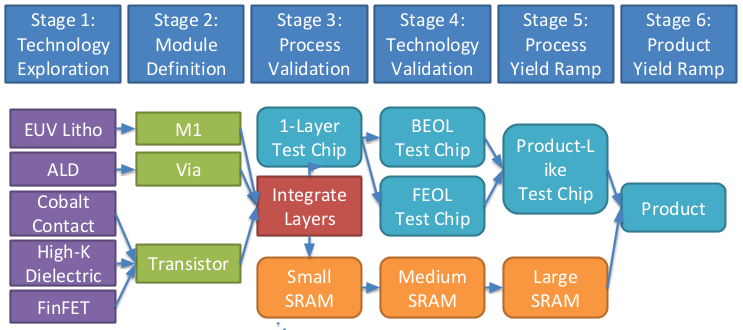
\includegraphics[width=3in]{lcv_flow}
	\caption{A typical technology development process with six stages}
	\label{fig_flow}
\end{figure}


Once these techniques have been identified the next step is to group sequences of processing steps into discrete modules. Basic electrical measurements and electron microscopy are used to validate these process modules. After module definition is complete the next step is process validation, wherein the process modules are integrated and used to create simple single-layer and transistor test structures as well as small SRAMs. Defectivity is extremely high at this stage and often driven by systematic process sensitivities as well as random particles. Information from the test structures and SRAMs is crucial in reducing this defectivity through adjustment of the various process parameters.

The next step after process validation is technology validation. Integration continues, with more complex test structures targeted towards both the front end of the line (FEOL) and back end of the line (BEOL), as well as medium-sized SRAMs, fabricated. Defectivity remains high at this stage, and significant effort is put into driving it down using the results derived from these test structures. This emphasis on reducing defectivity continues as the technology approaches product viability in the next step, process yield learning. Larger SRAMs and other product-representative test structures are manufactured, including logic test chips such as the ones described in this work. The final step is product yield learning, wherein product designs are taped out and manufactured at reduced volumes. Initial product yield is expected to be low even with all of the previous emphasis on identifying and reducing process defectivity; it is crucial for the commercial viability of the technology that product yield losses be identified and corrected as quickly as possible before volume manufacturing begins.

\section{CM-LCV: an Alternative Perspective} \label{cm_lcv_background}
\textbf{This is the most important section of the paper and we need to have a concise summary of all relevant work on CM-LCV.}

\textit{Paragraph 3} - The desired properties of an LCV: regularity, design reflection, testability, and diagnosability

\textit{Paragraph 4} - The basic properties of a CM-LCV \cite{lcv_prop} (bijective function, c-testability, vh-bijectivity, and functional unit block) and their implications on testability and diagnosability

\textit{Paragraph 5} - The enhanced properties of a CM-LCV: 

	\begin{itemize}
		\item Design reflection \cite{lcv_reflect_1}\cite{lcv_reflect_2}\cite{lcv_reflect_3}\cite{lcv_reflect_4}
		\item BIST \cite{lcv_bist}
		\item Multiple-defect diagnosis \cite{lcv_mult}
		\item Path delay fault diagnosis?
	\end{itemize}
	
%\textbf{Figure}: \ref{fig_lcv_example}
%	
%\begin{figure}[h]
%	\centering
%	
\includegraphics[width=3in]{dummy}
%	\caption{Example of a CM-LCV}
%	\label{fig_lcv_example}
%\end{figure}

\section{Experiments} \label{exp}
%\textit{Paragraph 6} - This section provides an apple-to-apple comparison of the testability and diagnosability between conventional test chips and CM-LCVs. Specially, we perform fault simulation and logic-level diagnosis for different fault models on commercial test chips (ITC'99 b17 benchmark circuit and L2B cache controller), commercial test chips with DFT features (the two circuits described previously with inserted test points), and three CM-LCVs designed to maximize design reflection and fault coverage.

Here, the testability and diagnosability of several CM-LCVs are compared with benchmark circuits representing conventional test chips. Using a 65nm commercial standard cell library, the conventional test chips are synthesized from the ITC99 b17 benchmark circuit \cite{itc99} and the L2B cache controller of the OpenSPARC T2 processor after replacing their memory elements with extra input and output pins to make them fully combinational. Additionally, extra test points are inserted to the test chips to improve their testability. Specifically, for a given circuit, ATPG identifies the redundant faults in the circuit and the gates that cause them to be redundant; test points can then be inserted at these gates to make the redundant faults controllable or observable. To have a direct comparison with these test chips, several CM-LCVs are constructed to optimally reflect them while maintaining high fault coverage as described in Section \ref{cm_lcv_background}. In the experiments, each test chip is compared against its enhanced version with inserted test points (hence referred to as TPI) and three CM-LCVs with different degrees of design reflection.

\subsection{Experimental Setup} \label{exp_setup}
%\textit{Paragraph 7} - We use two state-of-the-art commercial test and diagnosis tools and the fault models of SSL, IP, open-wire, and layout-aware bridge in our experiments. Elaborate on the input-pattern fault model since the reader might be least familiar with it.

Appropriate fault modeling and a test set are needed to evaluate an IC's testability and diagnosability. While fault models are usually constructed at a high abstraction level and do not capture all possible defect behaviors in an IC, each fault model represents a set of assumptions about how defects affect a circuit under test. In the test literature, defects are usually modeled as structural modification of the circuit interconnect at the gate-level. However, it is also possible to model defects functionally by changing the circuit's functionality. Fault models can also be categorized to be static or dynamic. A static fault model assumes that the effect of the defect is permanent regardless of the IC's operating conditions. Dynamic fault models are more complicated and take into account of timing (i.e. clock speed), voltage, temperature, and other variables. This comparison is restrained to static faults and uses three structural fault models and one functional fault model: 

\subsubsection{Single Stuck-Line (SSL)} each defect is modeled as a signal line being permanently stuck at either a logic-0 or a logic-1. For a netlist with $n$ signal lines, there are $2n$ SSL faults.

\subsubsection{Open} each defect is modeled as a broken wire in the circuit netlist. While this fault model can model the defect behavior of every signal line in a circuit netlist, distinction should be made between the stem line and the branch lines when a signal line fans out into multiple gates. The open fault model is a subset of the SSL fault model since it assumes that the broken wire is permanently stuck at either logic-0 or logic-1, but unlike the more general SSL fault model, open faults can always be activated and fault simulation is not needed (\textbf{need more elaboration}). For a netlist with $n$ stem signal lines and $m$ branch signal lines, there are $m+n$ open faults.

\subsubsection{Bridge} each defect is modeled as an unintended connection between two signal lines and behaves as a short circuit. At the logical level, a bridge fault can be modeled in three ways: wired-and, in which a logic-0 in one signal line overrides a logic-1 in the other; wired-or, which behaves similarly to wired-and except that a logic-1 overrides a logic-0; and dominant, which assumes that one signal line "dominates" the other and its logic value always overrides that of the other signal line. To keep the fault model practical and enumerable, however, layout information should be used to identify the likely defect sites. For a netlist with $n$ pairs of likely bridge fault cites, there are $4n$ bridge faults: $n$ wired-and bridge faults, $n$ wired-or bridge faults, and $2n$  dominant bridge faults.

\begin{figure}[h]
	\centering
	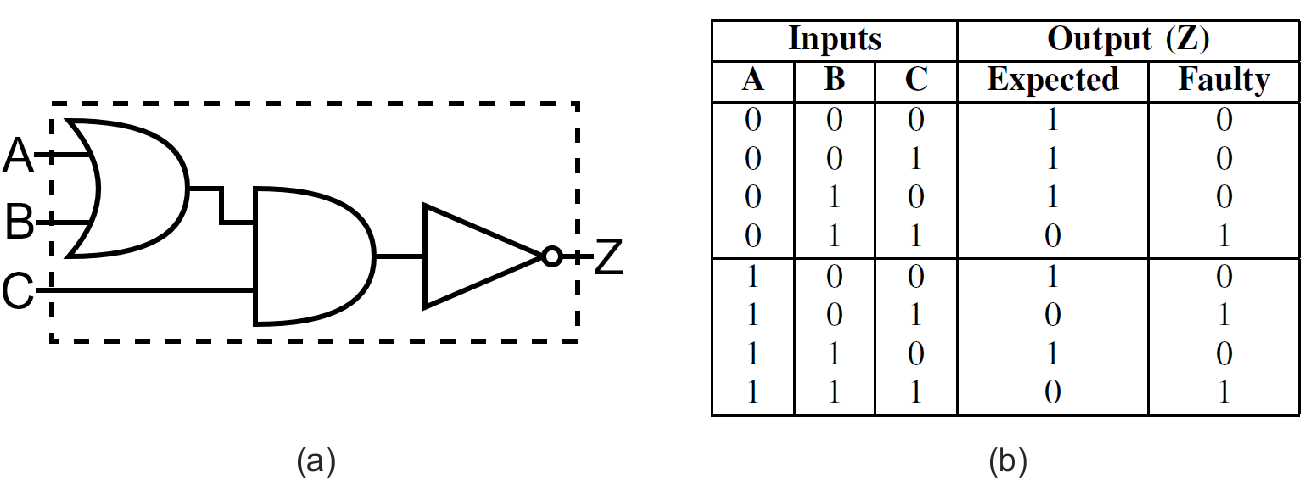
\includegraphics[width=3in]{ip_example}
	\caption{(a) Schematic of the standard-cell OAI21 (b) Truth table illustrating the IP fault model for the OAI21 standard-cell}
	\label{fig_fault_model}
\end{figure}

\subsubsection{Input Pattern (IP)} unlike the previous fault models which target the circuit interconnect, the Input Pattern (IP) fault model \cite{ip} allows a circuit module to arbitrarily change its functionality. The definition of circuit module is arbitrary, and work in \cite{ip} and \cite{gate_exhaustive} has shown that if applied at the standard-cell level, the IP fault model ensures the detection of every irredundant intra-cell defect. Figure \ref{fig_fault_model} illustrates how the IP fault model is applied to a simple 3-input standard cell, OAI21. Figure \ref{fig_fault_model}(a) shows the schematic of the standard-cell with inputs A, B, and C, and output Z. The rows of the truth table in Figure \ref{fig_fault_model}(b) form the input patterns of the standard-cell and are exhaustively enumerated as \textit{$ip_0$}=000, \textit{$ip_1$}=001, ... \textit{$ip_7$}=111. Each input pattern has an expected response and a faulty response as listed in the fourth and fifth columns of the truth table, respectively. The assumption of the IP fault model is that for a given input pattern, an intra-cell defect changes the standard-cell's response from the expected value to a faulty one. For example, the IP fault $f_0=(000 \rightarrow 1/0)$ denotes the standard-cell's functionality change for the first input pattern, where the first value after the arrow indicates the expected response and the second value is the faulty response. For a standard-cell with $n$ inputs, there are $2^n$ IP faults.

A high quality test set needs to provide high fault coverage for all fault models under consideration with reasonable size and test generation effort. While tests for the CM-LCVs are generated by leveraging the their C-testability as described in Section \ref{cm_lcv_background}, it is necessary to use an ATPG tool to generate tests for the product-like test chips. Commercial ATPG tools have been optimized to generate tests for SSL faults and usually support user-defined fault models, but a SSL test set alone is insufficient because it does not guarantee the detection of other faults. Additionally, it is inefficient to use the bridge fault model for test generation because of its limited fault activation and propagation conditions while the open fault model is a subset of the SSL fault model. Therefore, the IP fault model and the SSL fault model are used for test generation to effectively cover all fault models under consideration.

 % \textbf{TODO: update this paragraph after drafting the CM-LCV section (Section \ref{cm_lcv_background}).}

% Prior work in \cite{lcv_reflect_1} and \cite{lcv_mult} has shown that a CM-LCV is C-testable \cite{friedman}, a property that 


\textit{Paragraph 8} - We normalize the experimental results based on circuit size (standard cell count and I/O pin count) and test set size (custom test set for CM-LCVs and ATPG-generated test set for the commercial test chips).

\subsection{Experimental Results} \label{exp_results}
\textit{Paragraph 9} - Discuss the experimental results we obtain for the circuits under comparison: for each fault model, we compare each circuit's fault coverage and diagnostic callout (physical diagnostic resolution and an analysis of each circuit fault's failing patterns).

\textbf{Figures}: \ref{fig_diag_res}

\textbf{Tables}: \ref{table_coverage}

\begin{table*}[h]
	\caption{Fault coverage and diagnostic coverage of the circuits under comparison}
	\begin{center}
		\begin{tabular}{ |c|c|c|c|c|c|c|c| } 
			\hline
			 & ITC b17 & TPI b17 (50PI) & TPI b17 (100PI) & LCV b17 10k & LCV b17 20k & LCV b17 50k & L2B \\
			\hline
			\textbf{Total Standard Cells} & 13,139 & 14,425 & 14,425 & 9,519 & 10,216 & 9,936 & 7,678 \\ 
			\hline
			\textbf{I/O Pin Count} & 2,964 & 3,133 & 3,174 & 120 & 126 & 120 & 7,135 \\ 
			\hline
			\textbf{Test Set Size} & 1,335 & 1,246 & 1,155 & 512 & 512 & 512 & 1,681 \\
			\hline
			\textbf{Diagnostic Coverage} & & & & & & & \\
			\hline
			\multicolumn{8}{|c|}{\textbf{SSL Fault Model}} \\
			\hline
			\textbf{\# Faults} & 105,412 & 113,466 & 113,548 & 58,992 & 64,754 & 65,086 & 69,420 \\
			\textbf{Fault Coverage} & 99.99\% & 100\% & 100\% & 99.86\% & 99.96\% & 99.98\%  & 100\% \\
			%\textbf{Diagnostic Coverage} & 0.5755 & 0.5880 & 0.5879 & 0.4637 & 0.4820 & 0.5022 \\
			\hline
			
			\multicolumn{8}{|c|}{\textbf{IP Fault Model}} \\
			\hline
			\textbf{\# Faults} & 164,734 & 169,878 & 169,878 & 50,112 & 57,118 & 61,296 & 62,860 \\
			\textbf{Fault Coverage} & 62.24\% & 77.81\% & 78.01\% & 80.95\% & 78.59\% & 73.18\% & 78.48\% \\
			%\textbf{Diagnostic Coverage} & 0.6055 & 0.7679 & 0.7698 & 0.6858 & 0.6753 & 0.6507 \\
			\hline
			
			\multicolumn{8}{|c|}{\textbf{Open Fault Model}} \\
			\hline
			\textbf{\# Faults} & 20,998 & 22,503 & 22,564 & 12,998 & 14,303 & 14,500 & 13,932 \\
			\textbf{Fault Coverage} &  & 89.20\% &  &  & 99.12\% &  &  \\
			%\textbf{Diagnostic Coverage} & & & & & & \\
			\hline
			
			\multicolumn{8}{|c|}{\textbf{Layout-Aware Bridge Fault Model}} \\
			\hline
			\textbf{\# Faults} & 376,768 & 331,076 & 340,956 & 78,196 & 94,664 & 98,300 & 269,940 \\
			\textbf{Fault Coverage} & & & & & 92.54\% & &  \\
			%\textbf{Diagnostic Coverage} & & & & & & \\
			\hline
			
		\end{tabular}
	\end{center}
	\label{table_coverage}
\end{table*}

\begin{figure}[h]
	\centering
	
\includegraphics[width=3in]{dummy}
	\caption{Diagnostic callout analysis}
	\label{fig_diag_res}
\end{figure}

\textit{Paragraph 10} - Introduce the concepts of fault signature and diagnostic coverage \cite{lcv_diag} and provide additional comparisons in light of these two concepts. 

\textbf{Figures}: \ref{fig_fault_sig}

\begin{figure}[h]
	\centering
	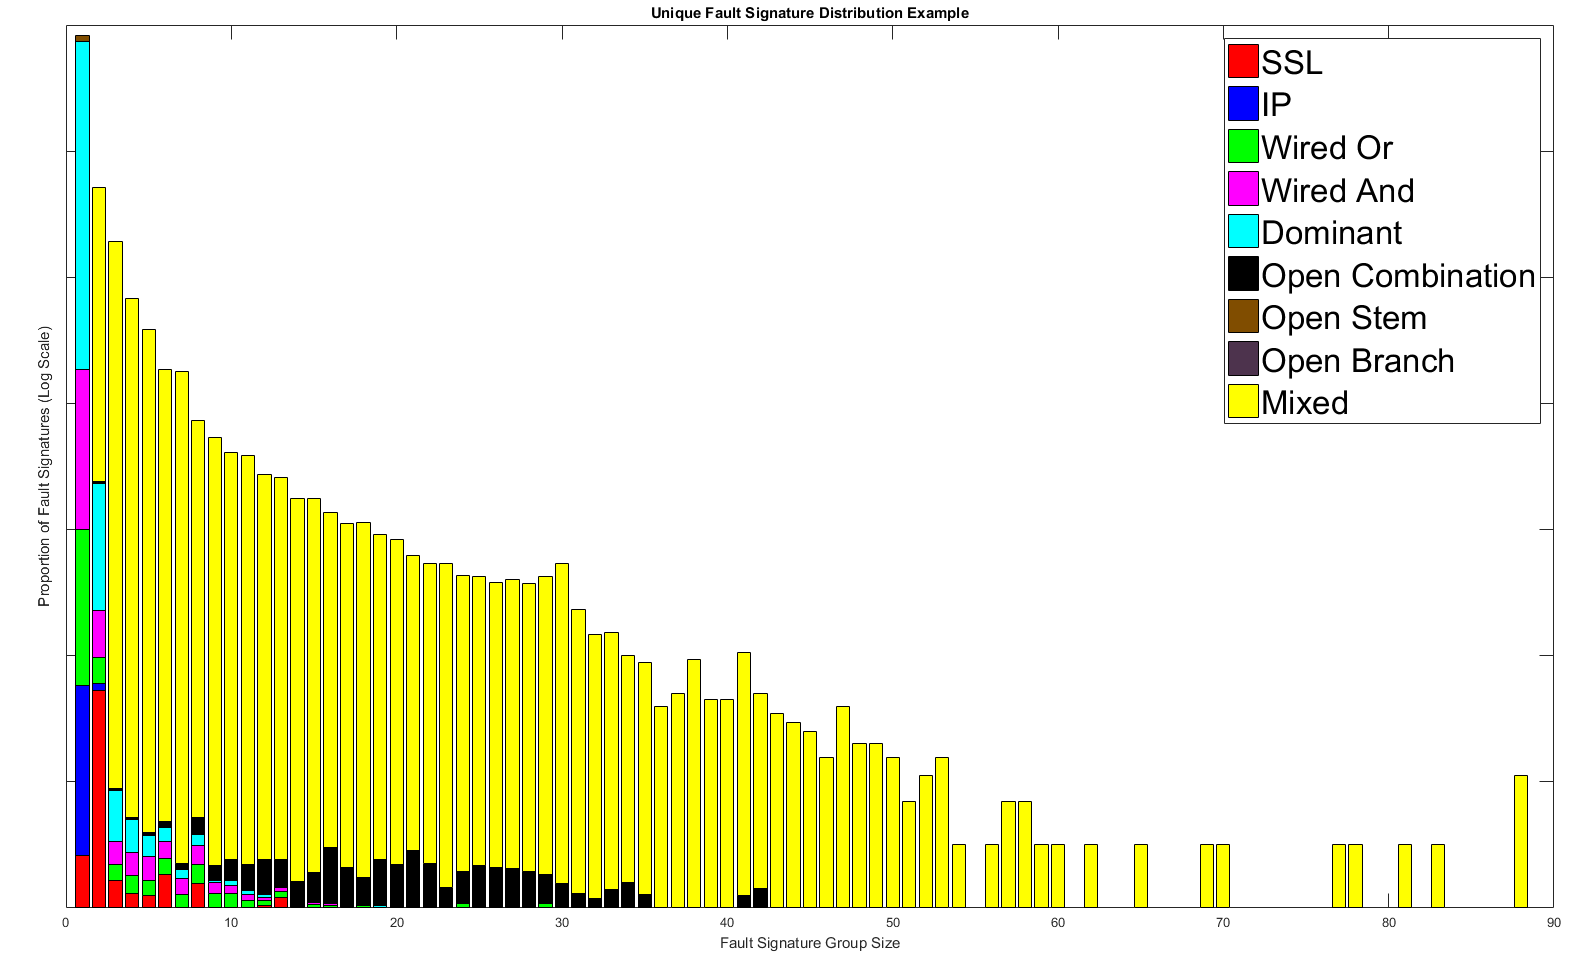
\includegraphics[width=3in]{fault_sig}
	\caption{Unique fault signatures distribution}
	\label{fig_fault_sig}
\end{figure}

\section{Summary} \label{summary}
\textit{Paragraph 11} - Summarize the comparison and talk about the current work at ACTL:
	\begin{itemize}
		\item Over 60 LCV designs are in production in three different fabrication facilities
		\item We are applying custom diagnosis to a large volume of failing LCVs that have been fabricated in some state-of-the-art facilities 
	\end{itemize}

% needed in second column of first page if using \IEEEpubid
%\IEEEpubidadjcol

% An example of a floating figure using the graphicx package.
% Note that \label must occur AFTER (or within) \caption.
% For figures, \caption should occur after the \includegraphics.
% Note that IEEEtran v1.7 and later has special internal code that
% is designed to preserve the operation of \label within \caption
% even when the captionsoff option is in effect. However, because
% of issues like this, it may be the safest practice to put all your
% \label just after \caption rather than within \caption{}.
%
% Reminder: the "draftcls" or "draftclsnofoot", not "draft", class
% option should be used if it is desired that the figures are to be
% displayed while in draft mode.
%
%\begin{figure}[!t]
%\centering
%\includegraphics[width=2.5in]{myfigure}
% where an .eps filename suffix will be assumed under latex, 
% and a .pdf suffix will be assumed for pdflatex; or what has been declared
% via \DeclareGraphicsExtensions.
%\caption{Simulation Results}
%\label{fig_sim}
%\end{figure}

% Note that IEEE typically puts floats only at the top, even when this
% results in a large percentage of a column being occupied by floats.


% An example of a double column floating figure using two subfigures.
% (The subfig.sty package must be loaded for this to work.)
% The subfigure \label commands are set within each subfloat command, the
% \label for the overall figure must come after \caption.
% \hfil must be used as a separator to get equal spacing.
% The subfigure.sty package works much the same way, except \subfigure is
% used instead of \subfloat.
%
%\begin{figure*}[!t]
%\centerline{\subfloat[Case I]\includegraphics[width=2.5in]{subfigcase1}%
%\label{fig_first_case}}
%\hfil
%\subfloat[Case II]{\includegraphics[width=2.5in]{subfigcase2}%
%\label{fig_second_case}}}
%\caption{Simulation results}
%\label{fig_sim}
%\end{figure*}
%
% Note that often IEEE papers with subfigures do not employ subfigure
% captions (using the optional argument to \subfloat), but instead will
% reference/describe all of them (a), (b), etc., within the main caption.


% An example of a floating table. Note that, for IEEE style tables, the 
% \caption command should come BEFORE the table. Table text will default to
% \footnotesize as IEEE normally uses this smaller font for tables.
% The \label must come after \caption as always.
%
%\begin{table}[!t]
%% increase table row spacing, adjust to taste
%\renewcommand{\arraystretch}{1.3}
% if using array.sty, it might be a good idea to tweak the value of
% \extrarowheight as needed to properly center the text within the cells
%\caption{An Example of a Table}
%\label{table_example}
%\centering
%% Some packages, such as MDW tools, offer better commands for making tables
%% than the plain LaTeX2e tabular which is used here.
%\begin{tabular}{|c||c|}
%\hline
%One & Two\\
%\hline
%Three & Four\\
%\hline
%\end{tabular}
%\end{table}


% Note that IEEE does not put floats in the very first column - or typically
% anywhere on the first page for that matter. Also, in-text middle ("here")
% positioning is not used. Most IEEE journals use top floats exclusively.
% Note that, LaTeX2e, unlike IEEE journals, places footnotes above bottom
% floats. This can be corrected via the \fnbelowfloat command of the
% stfloats package.

% if have a single appendix:
%\appendix[Proof of the Zonklar Equations]
% or
%\appendix  % for no appendix heading
% do not use \section anymore after \appendix, only \section*
% is possibly needed

% use appendices with more than one appendix
% then use \section to start each appendix
% you must declare a \section before using any
% \subsection or using \label (\appendices by itself
% starts a section numbered zero.)
%


%\appendices
%\section{Proof of the First Zonklar Equation}
%Some text for the appendix.

% use section* for acknowledgement
%\section*{Acknowledgment}
%The authors would like to thank...


% Can use something like this to put references on a page
% by themselves when using endfloat and the captionsoff option.
\ifCLASSOPTIONcaptionsoff
  \newpage
\fi



% trigger a \newpage just before the given reference
% number - used to balance the columns on the last page
% adjust value as needed - may need to be readjusted if
% the document is modified later
%\IEEEtriggeratref{8}
% The "triggered" command can be changed if desired:
%\IEEEtriggercmd{\enlargethispage{-5in}}

% references section

% can use a bibliography generated by BibTeX as a .bbl file
% BibTeX documentation can be easily obtained at:
% http://www.ctan.org/tex-archive/biblio/bibtex/contrib/doc/
% The IEEEtran BibTeX style support page is at:
% http://www.michaelshell.org/tex/ieeetran/bibtex/
%\bibliographystyle{IEEEtran}
% argument is your BibTeX string definitions and bibliography database(s)
%\bibliography{IEEEabrv,../bib/paper}
%
% <OR> manually copy in the resultant .bbl file
% set second argument of \begin to the number of references
% (used to reserve space for the reference number labels box)
\begin{thebibliography}{1}

	\bibitem{test_struct_1}
	M. B. Buehler, \emph{Microelectronic Test Chips for VLSI Electronics, VLSI Electronics Microstructure Science}, vol. 6, Chap. 9, pp. 529 - 576, Academic Press, 1983.
	
	\bibitem{test_struct_2}
	J. E. Nelson et al., ``Extraction of Defect Density and Size Distribution from Product ICs,'' \emph{IEEE Design \& Test of Computers}, pp. 390 - 400, May 2006.
	
	\bibitem{test_struct_3}
	J. E. Nelson et al., ``Extraction of Defect Density and Size Distributions from Wafer Sort Test Results,'' \emph{Design, Automation and test in Europe}, pp. 1 - 6, 2006.
	
	
	\bibitem{sram}
	M. Fujii et al., ``A Large Scale, Flip-Flop RAM Imitating a Logic LSI for Fast Development of 	Process Technology,'' \emph{Microelectronic Test Structures}, pp. 131-134, 2007.
	
	\bibitem{pdf}
	C. Hess et al., ``Logic Characterization Vehicle to Determine Process Variation Impact on Yield and Performance of Digital Circuits,'' \emph{Microelectronic Test Structures}, pp. 189-196, 2002.
	
	\bibitem{lcv_prop}
	R. D. Blanton, B. Niewenhuis, and C. Taylor, ``Logic Characterization Vehicle design for Maximal Information Extraction for Yield Learning,'' \emph{International Test Conference}, pp. 1–10, Oct 2014.
	
	\bibitem{lcv_reflect_1}
	R. D. Blanton, B. Niewenhuis, and Z. Liu, ``Design Reflection for Optimal Test-Chip Implementation,'' \emph{International Test Conference}, pp. 1 - 10, 2015.
	
	\bibitem{lcv_reflect_2}
	Z. Liu, B. Niewenhuis, S., Mittal, and R. D. Blanton, ``Achieving 100\% Cell-Aware Coverage by Design,'' \emph{Design, Automation \& Test in Europe}, pp. 109 - 114, 2016.
	
	\bibitem{lcv_reflect_3}
	P. Fynan et al., ``Logic Charaterization Vehicle Design Reflection via Layout Rewiring,'' \emph{International Test Conference}, pp. 1 - 10, 2016.
	
	\bibitem{lcv_reflect_4}
	Z. Liu, P. Fynan, and R. D. Blanton, ``Front-End Layout Reflection for Test Chip Design,'' \emph{International Test Conference}, pp. 1 - 10, 2017.
	
	\bibitem{lcv_bist}
	B. Niewenhuis, and R. D. Blanton, ``Efficient Built-In Self Test of Regular Logic Characterization Vehicles,'' \emph{VLSI Test Symposium}, pp. 1 - 6, 2015.
	
	\bibitem{lcv_mult}
	B. Niewenhuis, S. Mittal, and R. D. Blanton, ``Multiple-Defect Diagnosis for Logic Characterization Vehicles,'' \emph{European Test Symposium}, pp. 1 - 6, 2017.

	\bibitem{lcv_diag}
	S. Mittal, Z. Liu, B. Niewenhuis, and R. D. Blanton, ``Test Chip Design for Optimal Cell-Aware Diagnosability,'' \emph{International Test Conference}, pp. 1 - 8, 2016.
	
	\bibitem{itc99}
	S. Davidson, ``ITC'99 Benchmark Circuits-Preliminary Results,'' \emph{International Test Conference}, pp 1125 - 1130, 1999.
	
	\bibitem{t2}
	Oracle.com. (2018). \emph{OpenSPARC T2}. [online] http://www.oracle.com/technetwork/systems/opensparc/opensparc-t2-page-1446157.html [Accessed 9 Jan. 2018].
	
	\bibitem{ip}
	R. D. Blanton and J. P. Hayes, ``Properties of the Input Pattern Fault Model,'' \emph{IEEE International Conference on Computer Design}, Oct. 1997.
	
	\bibitem{gate_exhaustive}
	K. Y. Cho, S. Mitra, and E. McCluskey, ``Gate Exhaustive Testing'', \emph{IEEE International Test Conference}, Nov. 2005.
	
	\bibitem{friedman}
	A. D. Friedman, ``Easily Testable Iterative Systems'', \emph{IEEE Transactions on Computers}, vo. C-22, np. 12, pp. 1061 - 1064, Dec. 1973.

\end{thebibliography}

% biography section
% 
% If you have an EPS/PDF photo (graphicx package needed) extra braces are
% needed around the contents of the optional argument to biography to prevent
% the LaTeX parser from getting confused when it sees the complicated
% \includegraphics command within an optional argument. (You could create
% your own custom macro containing the \includegraphics command to make things
% simpler here.)
%\begin{biography}[{\includegraphics[width=1in,height=1.25in,clip,keepaspectratio]{mshell}}]{Michael Shell}
% or if you just want to reserve a space for a photo:

%\begin{IEEEbiography}[{\includegraphics[width=1in,height=1.25in,clip,keepaspectratio]{picture}}]{John Doe}
%\blindtext
%\end{IEEEbiography}

% You can push biographies down or up by placing
% a \vfill before or after them. The appropriate
% use of \vfill depends on what kind of text is
% on the last page and whether or not the columns
% are being equalized.

%\vfill

% Can be used to pull up biographies so that the bottom of the last one
% is flush with the other column.
%\enlargethispage{-5in}



% that's all folks
\end{document}


